\documentclass[11pt]{article}
\usepackage[a4paper,margin=26mm]{geometry}
\usepackage[T1]{fontenc}
\usepackage{lmodern,microtype,amsmath,amssymb,amsthm,mathtools}
\usepackage{graphicx,booktabs,array,xcolor}
\usepackage[numbers,sort&compress]{natbib}
\usepackage{enumitem}
\usepackage[colorlinks=true,linkcolor=blue!45!black,citecolor=blue!45!black,urlcolor=blue!45!black]{hyperref}
\allowdisplaybreaks
\setlist{itemsep=2pt,topsep=4pt}
\newtheorem{theorem}{Theorem}[section]
\newtheorem{proposition}[theorem]{Proposition}
\newtheorem{lemma}[theorem]{Lemma}
\newtheorem{corollary}[theorem]{Corollary}
\theoremstyle{definition}
\newtheorem{definition}[theorem]{Definition}
\newtheorem{remark}[theorem]{Remark}
\newcommand{\R}{\mathbb R}
\newcommand{\C}{\mathbb C}
\newcommand{\N}{\mathbb N}
\newcommand{\T}{\mathbb T}
\newcommand{\Rea}{\operatorname{Re}}
\newcommand{\Ree}{\operatorname{Re}}
\newcommand{\norm}[1]{\left\lVert#1\right\rVert}
\newcommand{\abs}[1]{\left\lvert#1\right\rvert}
\newcommand{\pos}[1]{\left(#1\right)_+}
\newcommand{\dd}{\,\mathrm d}
\hypersetup{
 pdftitle={Near-edge extrapolation and parabolic smoothing in exact Navier-Stokes shear flows},
 pdfauthor={C. K. Zeng},
 pdfsubject={Localized signed fluxes of finite-mode periodic shear flows},
 pdfkeywords={Navier-Stokes, exponential sums, extrapolation, Chebyshev polynomials, heat flow}
}
\title{Near-edge extrapolation and parabolic smoothing\\
in exact Navier--Stokes shear flows}
\author{C. K. Zeng\thanks{Independent Researcher.
ORCID: \href{https://orcid.org/0009-0002-5402-3374}{0009-0002-5402-3374}.}}
\date{5 September 2026}
\begin{document}
\maketitle

\begin{abstract}
I study the signed transport flux through a thin radial collar for exact
periodic Navier--Stokes shears whose nonconstant component has \(q\)
positive Fourier frequencies in one dyadic band. A local reconstruction
of a near-edge estimate for exponential sums gives a bound by the
two-thirds power of the space--time cubic mass of that component on the
full central plateau. The coefficient has the form
\(C a^{2/3}R^{-1/3}q^7
\exp(20\sqrt2\,q\sqrt{(\delta+\delta_0)/(a-\delta_0)})\);
it is uniform in the carrier frequency, amplitudes, phases, and constant
transport speed. A time-weighted estimate for decaying exponential sums
supplies the high-frequency part of the argument.

Real dyadic packets retain both linear endpoint growth and the
\(\exp(cq\sqrt d)\) spatial extrapolation scale. They can be realized by
integer-mode heat shears at a prescribed time. I then analyze one
start-prepaid Chebyshev family over the complete time interval. In the
joint regime \(m/\sqrt A\to\infty\), \(m/A^2\to0\), the quotient of its
positive integrated collar flux by the two-thirds power of the full-plateau
mass, multiplied by \(R^{1/3}\), has an edge-dependent factor of order
\(\exp(\Theta((m^2/A)^{1/3}))\), up to explicit algebraic factors.
The static edge scale is \(\exp(\Theta(m/\sqrt A))\).
The general extrapolation scale is established in prior work; the focus
here is its realization and interaction with this local observable.
The results concern smooth exact shears and do not give a regularity
criterion for general weak solutions.
\end{abstract}

\medskip
\noindent\textbf{2020 Mathematics Subject Classification.}
35Q30, 41A17, 35K05, 76D05.

\noindent\textbf{Keywords.}
Navier--Stokes shear flow; localized signed flux; exponential sum;
near-edge extrapolation; Chebyshev polynomial; heat equation.

\section{Introduction}
\label{sec:introduction}

Spatial concentration and diffusion affect a local observation in
different ways. An oscillatory profile can be small on an observed
interval and large just outside it. During its heat evolution, the
size and location of this contrast change. For a signed transport flux,
the signs on the two sides of the observation region matter as well.
This paper separates these effects in a class for which the velocity
field and its evolution are explicit.

On \(\T^3=(\R/2\pi\mathbb Z)^3\), consider
\[
 u(t,x)=(0,B,F(t,x_2)),\qquad
 \partial_tF+B\partial_{x_2}F-\partial_{x_2}^2F=0 .
\]
With constant pressure this solves the unforced incompressible
Navier--Stokes equations with unit viscosity. Each finite trigonometric
initial profile gives a smooth periodic solution for all positive time.
Exact plane shears and more general shearing waves are classical;
see Singh and Sridhar~\cite{SinghSridhar2017}. The question here is how
much signed quadratic transport can cross a thin spherical collar,
compared with the cubic mass of \(F\) on its central plateau, over the
same complete time interval.

Three statements are useful, but have different quantifiers.
A uniform upper estimate applies to every finite packet in the dyadic
class. A sharp spatial witness may be chosen to fit one prescribed
observation time. A lower bound for a time-integrated signed flux must
instead use one initial datum throughout the interval and control the
full plateau, including its caps. A spatial witness by itself does not
settle the last question.

\paragraph{The spatial input.}
Near-edge extrapolation for sparse Fourier sums has recently been
studied by Zhang~\cite{Zhang2026}. The scale
\(N\exp(CN\sqrt d)\) near an interval endpoint and its exponential
sharpness belong to that work. The local proof below follows its
orthogonal-basis and half-line comparison architecture, with
attribution. I include the finite-range argument and explicit constants
to make the analytic dependence of the collar estimate transparent.
Two other inputs are the endpoint and derivative inequalities recorded
by Erd\'elyi~\cite{Erdelyi2017}. They are stated with their hypotheses
where they enter the proof.

\paragraph{The shear-flow estimates.}
The first result controls the complete signed flux by the full-plateau
mass, uniformly in the transport speed and frequency positions.
The proof combines spatial extrapolation with a four-term energy
identity. A time-weighted exponential-sum lemma handles the onset of
the time cutoff at high carrier frequency. Its proof uses a
frequency-uniform decaying basis and an initial interval of length
proportional to the number of terms.

The next result realizes polynomial endpoint witnesses in the real
dyadic Fourier class. A real-rooted polynomial has no vanishing
coefficient in the confluent Fourier representation at any positive
confluence parameter. This strengthens the small-parameter
nonvanishing argument. Approximation errors remain a separate issue
when the degree increases.

A joint degree--scale heat asymptotic then describes one Chebyshev
witness over the entire interval. The common heat amplitude has
logarithmic size \((m^2/A)^{2/3}\), while the relative edge tilt has size
\((m^2/A)^{1/3}\). The proof keeps this relative tilt, the terminal time
layer, signed pairing, and full-plateau cross-section weights.

Heat evolution on polynomial spaces is a classical finite algebraic
operation. Recent work of Hall and Ho~\cite{HallHo2025} studies its
large-degree root distributions and random-matrix connections.
The observable considered here is different: a relative endpoint
amplitude and its contribution to a signed local shear flux.
Neither the heat operator on polynomials nor its finite series
representation is claimed as new.

\paragraph{Scope and organization.}
The Navier--Stokes statements are for exact periodic shears with
constant transport and finitely many integer modes. Constants can be
uniform across this family even though its initial energy is not
uniform across a sequence of witnesses. The cubic mass is the mass of
the third component \(F\), with the constant drift \(B\) excluded.
\emph{Full plateau} specifies the spatial integration region, not all
three velocity components. The planar extension on \(\R^3\) generally
has infinite total energy.

The next sections give the complete upper-bound proof, spatial
sharpness, and parabolic calculation. Quantitative consequences, a
finite diagnostic, and limitations follow. The accompanying audit
files record the research-note provenance and supplementary work.

\section{A uniform bound for the complete collar flux}
\label{sec:upper-bound}

The spatial estimate in this section holds for arbitrary real frequencies.
The passage to a heat-flow estimate uses the additional assumption that
the frequencies lie in one dyadic band.  The proof of the spatial estimate
follows the half-plane and Laguerre-polynomial approach of
Zhang~\cite{Zhang2026}.  The details, including the finite-range step, are
given below.  The constants are chosen for a short proof.

\subsection{A finite-dimensional half-plane basis}

For distinct complex numbers $\zeta_1,\ldots,\zeta_N$ with
$b_j=\operatorname{Re}\zeta_j>0$, consider the space spanned by
$e^{-\zeta_jt}$ in $L^2(0,\infty)$.  The Laplace transform, with boundary
norm $(2\pi)^{-1}\int_{\mathbb R}|\widehat h(i\xi)|^2\,d\xi$, is an
isometry on this space by Fourier Plancherel.  A useful orthonormal basis
has transforms
\begin{equation}\label{eq:ub-basis}
 \widehat\varphi_j(s)=\frac{\sqrt{2b_j}}{s+\zeta_j}
       \prod_{r<j}\frac{s-\overline{\zeta_r}}{s+\zeta_r},
 \qquad 1\le j\le N.
\end{equation}
Here and below inner products are linear in the first argument.
To verify this assertion, note that each factor in the product has
modulus one on the imaginary axis.  The kernel
$k_w(s)=(s+\overline w)^{-1}$ satisfies
\[
 \langle H,k_w\rangle=H(w),\qquad
 \|k_w\|^2=(2\operatorname{Re}w)^{-1}.
\]
These identities follow by applying Plancherel to
$e^{-\overline w t}$.  The norm of every vector in
\eqref{eq:ub-basis} is therefore one.  In the inner product of the $j$th
and $\ell$th vectors, $\ell<j$, cancel their common initial factors.
The remaining $j$th factor vanishes at $\overline{\zeta_\ell}$, so the
reproducing identity gives orthogonality.  Partial fractions show that
the first $j$ vectors lie in the span of the first $j$ kernels.  The
coefficient at $(s+\zeta_j)^{-1}$ is nonzero, since
$\zeta_r-\zeta_j\ne0$ and $\operatorname{Re}(\zeta_j+
\overline{\zeta_r})>0$.  This proves spanning as well.

Let
\[
 (V_\zeta h)(t)=\int_0^t e^{-\zeta(t-u)}h(u)\,du.
\]
Inverting the factors in \eqref{eq:ub-basis} gives
\begin{equation}\label{eq:ub-volterra}
 \varphi_j=
 \prod_{r<j}(I-2b_rV_{\zeta_r})
       \bigl(\sqrt{2b_j}e^{-\zeta_jt}\bigr).
\end{equation}
These are identities between entire exponential sums, so the same formula
holds at negative real times, with each integral oriented from $0$ to $t$.

Write
\[
 L_m(-y)=\sum_{\ell=0}^m\binom m\ell\frac{y^\ell}{\ell!},
 \qquad y\ge0.
\]
The elementary bound
\begin{equation}\label{eq:ub-laguerre}
 0\le L_m(-y)
 \le\sum_{\ell\ge0}\frac{(my)^\ell}{(\ell!)^2}
 \le\cosh(2\sqrt{my})\le e^{2\sqrt{my}}
\end{equation}
follows from $\binom{2\ell}{\ell}\le4^\ell$.  In particular, if all
$b_j=\beta/2$, expansion of \eqref{eq:ub-volterra} over subsets gives
\begin{equation}\label{eq:ub-basis-majorants}
 \begin{split}
 |\varphi_j(t)|&\le\sqrt\beta e^{-\beta t/2}
                         L_{j-1}(-\beta t),\quad t\ge0,\\
 |\varphi_j(-x)|&\le\sqrt\beta e^{\beta x/2}
                         L_{j-1}(-\beta x),\quad x\ge0.
 \end{split}
\end{equation}
For each subset with $\ell$ factors, the convolution simplex has volume
$t^\ell/\ell!$ or $x^\ell/\ell!$.  Equality of the real parts supplies
the common exponential factor; taking absolute values removes the signs
of the Volterra factors.  There are $\binom{j-1}{\ell}$ such subsets.

\subsection{Bilateral near-edge extrapolation}

\begin{theorem}[Near-edge estimate]\label{thm:ub-edge}
Let $N\ge1$ and
$g(x)=\sum_{j=1}^N c_je^{i\mu_jx}$, with $c_j\in\mathbb C$ and
$\mu_j\in\mathbb R$.  For every $d\ge0$,
\begin{equation}\label{eq:ub-edge}
 \max\{|g(1+d)|,|g(-1-d)|\}
 \le \sqrt{\frac{250}{19}}\,N
       e^{5\sqrt2N\sqrt d}\|g\|_{L^2(-1,1)}.
\end{equation}
The bound has no frequency-separation hypothesis.
\end{theorem}

\begin{proof}
Zero coefficients can be removed and repeated frequencies merged.  The
result with the resulting number of terms implies the stated bound, so
assume that all $N$ frequencies are distinct.  The zero function is
immediate.  For any $N$-term real-frequency exponential sum $F$ and
$\beta>0$, put
\[
 I_\beta(F)=\int_0^\infty|F(t)|^2e^{-\beta t}\,dt,
 \qquad H(t)=e^{-\beta t/2}F(t).
\]
Expand $H$ in \eqref{eq:ub-basis}, with
$\zeta_j=\beta/2-i\mu_j$.  Cauchy--Schwarz and
\eqref{eq:ub-basis-majorants} yield
\[
 |F(t)|^2e^{-\beta t}
 \le I_\beta(F)\,\beta e^{-\beta t}
              \sum_{j=1}^N L_{j-1}(-\beta t)^2.
\]
Consequently, by \eqref{eq:ub-laguerre},
\begin{align*}
 I_\beta(F)^{-1}\int_{25N/\beta}^\infty
             |F(t)|^2e^{-\beta t}\,dt
 &\le N\int_{25N}^\infty e^{-y+4\sqrt{Ny}}\,dy\\
 &\le N\int_{25N}^\infty e^{-y/5}\,dy
   =5Ne^{-5N}<\frac1{20}.
\end{align*}
The second inequality uses $4\sqrt{Ny}\le4y/5$ for $y\ge25N$.
It follows that
\begin{equation}\label{eq:ub-finite-range}
 I_\beta(F)\le\frac{20}{19}
       \int_0^{25N/\beta}|F(t)|^2e^{-\beta t}\,dt.
\end{equation}
At a negative time, the second bound in
\eqref{eq:ub-basis-majorants} instead gives
\[
 |F(-x)|^2\le\beta\sum_{j=1}^N L_{j-1}(-\beta x)^2 I_\beta(F).
\]
The factor $e^{\beta x}$ cancels because
$H(-x)=e^{\beta x/2}F(-x)$.

Take $F(t)=g(1-t)$, $x=d$, and $\beta=25N/2$.  The truncation point
in \eqref{eq:ub-finite-range} is $2$, and
\[
 |g(1+d)|^2
 \le\frac{20}{19}\frac{25N}{2}
       N e^{10\sqrt2N\sqrt d}\int_{-1}^1|g(x)|^2\,dx.
\]
Taking square roots proves the right endpoint bound.  Apply the same
argument to $g(-x)$ for the left endpoint.
\end{proof}

An affine consequence will be useful.  If $J=[-e,e]$, $e>0$, and
$I=[-e(1+d),e(1+d)]$, then
\begin{equation}\label{eq:ub-affine-edge}
 \|g\|_{L^\infty(I)}^2
 \le\frac{250}{19e}N^2e^{10\sqrt2N\sqrt d}
                  \int_J|g|^2.
\end{equation}
The theorem proves this outside $J$ and at its endpoints.  For an interior
point $z$, apply the $d=0$ assertion to $[-e,z]$ and $[z,e]$.  If the
two lengths are $\ell_-$ and $\ell_+$, the resulting inequalities are
$\ell_\pm|g(z)|^2\le(500/19)N^2\int_{J_\pm}|g|^2$.
Adding them and using $\ell_-+\ell_+=2e$ proves
\eqref{eq:ub-affine-edge} there as well.

\subsection{A time-weighted estimate}

\begin{lemma}[Time-weighted decay]\label{lem:ub-delay}
Let $(E,\mu)$ be a measure space, and let
$\zeta_1,\ldots,\zeta_N\in\mathbb C$ satisfy
$1\le\operatorname{Re}\zeta_j\le4$.  For measurable finite
coefficients $c_j(z)$, define
\[
 f(t,z)=\sum_{j=1}^N c_j(z)e^{-\zeta_jt},\qquad
 k(t)=\int_E|f(t,z)|^3\,d\mu(z),\qquad
 K_T=\int_0^T k(t)\,dt.
\]
For every $T>0$ with $K_T<\infty$,
\begin{equation}\label{eq:ub-delay}
 \int_0^T t\,k(t)^{2/3}\,dt\le C N^{4/3}K_T^{2/3},
\end{equation}
where $C$ is absolute.
\end{lemma}

\begin{proof}
Merge coincident exponents, retaining the notation $N$ for their number.
In \eqref{eq:ub-volterra}, $1\le b_j\le4$.  Every convolution over
$\ell$ factors is bounded by $e^{-t}t^\ell/\ell!$, while $2b_j\le8$.
Therefore
\[
 |\varphi_j(t)|\le\sqrt8 e^{-t}L_{j-1}(-8t)
              \le\sqrt8 e^{-t+2\sqrt{8Nt}}.
\]
For almost every $z$, set $I_b(z)=\int_0^b|f(t,z)|^2\,dt$.
The coefficients are finite, so $I_\infty(z)<\infty$.
Expansion in the orthonormal basis gives
\[
 |f(t,z)|^2\le8N e^{-2t+4\sqrt{8Nt}}I_\infty(z).
\]
Take $S=128N$.  For $t\ge S$ the exponent is at most $-t$, so
\[
 \int_S^\infty|f(t,z)|^2\,dt
 \le8Ne^{-S}I_\infty(z)<\tfrac12 I_\infty(z).
\]
Thus $I_\infty\le2I_S$ and
$|f(t,z)|^2\le16Ne^{-t}I_S(z)$ for $t\ge S$.

Suppose $T\ge S$.  Minkowski's integral inequality in $L^{3/2}(E)$
and H\"older's inequality in time imply
\[
 \|I_S\|_{L^{3/2}(E)}
 \le\int_0^S k(u)^{2/3}\,du\le S^{1/3}K_T^{2/3}.
\]
Hence $k(t)^{2/3}\le16NS^{1/3}e^{-t}K_T^{2/3}$ for $t\ge S$,
and the tail contributes at most
$16NS^{1/3}(S+1)e^{-S}K_T^{2/3}\le C N^{4/3}K_T^{2/3}$.
On the initial interval, H\"older gives
\[
 \int_0^{\min(T,S)}t\,k(t)^{2/3}\,dt
 \le\left(\int_0^{\min(T,S)}t^3\,dt\right)^{1/3}K_T^{2/3}
 \le4^{-1/3}S^{4/3}K_T^{2/3}.
\]
If $T<S$ this is already the whole integral.  These two cases prove the
lemma.  Reinstating the original number of exponents only increases its
right-hand side.
\end{proof}

The use of $I_S$ with $S=128N$ is essential to this argument.  Replacing
it by $I_T$ would introduce $T^{1/3}$ through H\"older's inequality and
would not establish the stated uniform bound.

For later use, suppose the temporal decay rates of $G(s,z)$ have real
parts in $[\lambda,4\lambda]$, and let
$h(s)=\int_E|G(s,z)|^3\,d\mu$ and $H=\int_0^4h(s)\,ds$.
If $0\le\eta(s)\le C_\eta s$, rescale $t=\lambda s$ in
\eqref{eq:ub-delay}.  Since $K_{4\lambda}=\lambda H$, this gives
\begin{equation}\label{eq:ub-cutoff-time}
 \lambda\int_0^4\eta(s)h(s)^{2/3}\,ds
 \le C C_\eta N^{4/3}\lambda^{-1/3}H^{2/3}.
\end{equation}

\subsection{The physical model and the uniform theorem}

Write $\mathbb T=\mathbb R/(2\pi\mathbb Z)$.  Fix
$0<\delta_0<\delta$ and a function
$\vartheta\in C_c^\infty((-\delta,\delta))$ such that
$0\le\vartheta\le1$ and $\vartheta=1$ on $[-\delta_0,\delta_0]$.
Fix also $\eta\in C^1([0,4])$ with
$0\le\eta\le1$ and $\eta(0)=0$.
For $R>0$, $a\ge\max(1,\delta+2\delta_0)$ and $(a+\delta)R<\pi/2$, set
\begin{align}
 \xi_{a,R}(x)&=\vartheta(|x|/R-a),&
 \mathcal S^{\rm plat}_{a,R}
 &=\{x\in\mathbb T^3:\,||x|/R-a|\le\delta_0\},
 \label{eq:ub-geometry}\\
 F(t,x_2)&=\sum_{j=1}^q A_je^{-n_j^2t}
                   \cos(n_jx_2-\phi_j-n_jBt),
 \label{eq:ub-F}
\end{align}
where $q\ge1$, $1\le n_1<\cdots<n_q\le2n_1$ are integers,
$A_j\ge0$, and $\phi_j,B\in\mathbb R$.
The support of the cutoff lies in a Euclidean chart of the torus, and it
is extended by zero outside that chart.  The field $u=(0,B,F)$ is an exact
smooth Navier--Stokes solution with viscosity one and pressure zero:
its only nonzero evolution equation is
$F_t+BF_{x_2}-F_{x_2x_2}=0$.

Define the complete flux and the full plateau observation by
\begin{align}
 \mathcal T_{\boldsymbol n,R}
 &=\frac12\int_0^{4R^2}\!\int_{\mathbb T^3}
       \eta(t/R^2)B\,\partial_2\xi_{a,R}(x)F(t,x_2)^2\,dx\,dt,
 \label{eq:ub-T}\\
 M^{\rm plat}_{\boldsymbol n,R}
 &=\int_0^{4R^2}\!\int_{\mathcal S^{\rm plat}_{a,R}}
                         |F(t,x_2)|^3\,dx\,dt.
 \label{eq:ub-M}
\end{align}
The time cutoff occurs in the flux; the plateau observation uses the
entire unweighted clock.

\begin{theorem}[Complete-clock upper bound]\label{thm:ub-flux}
For the data above, put
\[
 \Delta_a=\frac{\delta+\delta_0}{a-\delta_0},\qquad
 \Phi_a=20\sqrt2q\sqrt{\Delta_a}.
\]
There is a constant $C$, depending only on
$\vartheta,\delta_0,\delta$ and $\|\eta'\|_\infty$, such that
\begin{equation}\label{eq:ub-main-refined}
 |\mathcal T_{\boldsymbol n,R}|
 \le C a^{2/3}R^{-1/3}
       \left(q^4+\frac{q^7}{a^2}+q^{13/3}\right)e^{\Phi_a}
       \bigl(M^{\rm plat}_{\boldsymbol n,R}\bigr)^{2/3}.
\end{equation}
In particular,
\begin{equation}\label{eq:ub-main}
 |\mathcal T_{\boldsymbol n,R}|
 \le C a^{2/3}R^{-1/3}q^7e^{\Phi_a}
       \bigl(M^{\rm plat}_{\boldsymbol n,R}\bigr)^{2/3}.
\end{equation}
The constant is independent of $q,R$, all frequencies, amplitudes,
phases, and $B$.
\end{theorem}

\begin{proof}
Use the scaled variables
\[
 \begin{gathered}
 s=t/R^2,\quad z=x_2/(aR),\quad G(s,z)=F(R^2s,aRz),\\
 \kappa_j=n_jaR,\quad \alpha=\kappa_1,\quad
 v=BR/a,\quad\lambda=(\alpha/a)^2.
 \end{gathered}
\]
Then $G_s+vG_z-a^{-2}G_{zz}=0$, and its $2q$ complex spatial
frequencies are $\pm\kappa_j$, with $\alpha\le\kappa_j\le2\alpha$.
Let
\[
 \begin{gathered}
 e_a=1-\delta_0/a,\quad E_a=[-e_a,e_a],\quad
 I_a=[-1-\delta/a,1+\delta/a],\\
 h(s)=\int_{E_a}|G(s,z)|^3\,dz,\quad H=\int_0^4h(s)\,ds.
 \end{gathered}
\]
The assumptions imply $e_a\ge1/2$, $\Delta_a\le1$, and uniformly
bounded upper and lower lengths for these intervals.
Equation \eqref{eq:ub-affine-edge} with $N=2q$, followed by H\"older,
gives
\begin{equation}\label{eq:ub-observation}
 \|G(s)\|_{L^\infty(I_a)}^2
 \le\frac{1000}{19e_a}q^2e^{\Phi_a}\int_{E_a}|G|^2
 \le Cq^2e^{\Phi_a}h(s)^{2/3}.
\end{equation}

The following two estimates from the literature are used in the remaining
argument.  Erd\'elyi's Markov inequality~\cite{Erdelyi2017} states, for
$f(x)=\sum_{r=1}^N c_re^{i\mu_rx}$ on $[0,1]$, that
\begin{equation}\label{eq:ub-markov-input}
 \|f'\|_\infty\le C
       \left(N^5+\sum_{r=1}^N\mu_r^2\right)^{1/2}\|f\|_\infty.
\end{equation}
The more precise expression in that paper is
$(1+\varepsilon_N)(108N^5+\sum_r\mu_r^2)^{1/2}$, with a uniformly
bounded factor $1+\varepsilon_N$.
K\'os's endpoint inequality~\cite{Kos2008}, recorded in
Erd\'elyi's paper as (1.2), is
\begin{equation}\label{eq:ub-kos-input}
 |f(0)|\le2N\|f\|_{L^2(0,1)},\qquad
 f(r)=\sum_{j=1}^N c_je^{\gamma_jr},\quad
 \operatorname{Re}\gamma_j\ge0.
\end{equation}

Map $I_a$ affinely onto $[0,1]$ in
\eqref{eq:ub-markov-input}.  Its length is bounded above and below,
and $\sum_j(\kappa_j^2+(-\kappa_j)^2)\le8q\alpha^2$.
Together with \eqref{eq:ub-observation}, this proves
\begin{equation}\label{eq:ub-derivative}
 \|G_z(s)\|_{L^\infty(I_a)}^2
 \le C(q^7+q^3\alpha^2)e^{\Phi_a}h(s)^{2/3}.
\end{equation}
For fixed $z$, the function $r\mapsto G(4-r,z)$, $0\le r\le1$,
has at most $2q$ exponential terms with exponents
$(\kappa_j/a)^2\pm iv\kappa_j$.  Applying
\eqref{eq:ub-kos-input}, cubing, and using H\"older on the unit
interval yields
\begin{equation}\label{eq:ub-endpoint}
 h(4)\le64q^3\int_3^4h(s)\,ds\le64q^3H,
 \qquad h(4)^{2/3}\le16q^2H^{2/3}.
\end{equation}

The radial geometry can be computed exactly.  At $y=x_2$, the
cross-sectional integral of the cutoff is
$2\pi\int_{|y|}^\infty r\vartheta(r/R-a)\,dr$.
Differentiating with respect to $y$ gives
\[
 \int_{\mathbb T^2}\partial_2\xi_{a,R}(x_1,y,x_3)\,dx_1\,dx_3
 =-2\pi y\vartheta(|y|/R-a).
\]
Thus, with
\[
 W_a(z)=-2\pi az\vartheta(a(|z|-1)),\qquad
 \Xi_a(z)=\int_{-\infty}^zW_a(r)\,dr,
\]
the exact flux conversion is
\begin{equation}\label{eq:ub-flux-conversion}
 \mathcal T_{\boldsymbol n,R}
 =\frac{a^2R^3}{2}\,v\int_0^4\eta(s)
                         \int_{\mathbb R}W_a(z)G(s,z)^2\,dz\,ds.
\end{equation}
The function $W_a$ is odd and has zero integral.  Its two support
intervals have length $O(a^{-1})$, and $|W_a|\le Ca$ there.  Consequently
\begin{equation}\label{eq:ub-kernel-bounds}
 \operatorname{supp}\Xi_a\subset I_a,\qquad
 \|\Xi_a\|_1+\|\Xi_a\|_\infty\le C,\qquad
 \|\Xi_a''\|_1=\|W_a'\|_1\le Ca.
\end{equation}
These bounds follow directly by differentiating $W_a$ on its support;
that support stays away from $z=0$.

Put $\mathcal E(s)=\int_{\mathbb R}\Xi_a(z)G(s,z)^2\,dz$.
Multiplying
$(G^2)_s+v(G^2)_z-a^{-2}(G^2)_{zz}=-2a^{-2}|G_z|^2$
by $\Xi_a$, and then integrating in space and time, gives
\begin{align}
 v\int_0^4\eta\int W_aG^2
 &=\eta(4)\mathcal E(4)-\int_0^4\eta'\mathcal E\,ds
 \nonumber\\
 &\quad-a^{-2}\int_0^4\eta\int\Xi_a''G^2
       +2a^{-2}\int_0^4\eta\int\Xi_a|G_z|^2.
 \label{eq:ub-energy}
\end{align}
There is no initial-face term because $\eta(0)=0$.
Using \eqref{eq:ub-observation}, \eqref{eq:ub-endpoint}, and
\eqref{eq:ub-kernel-bounds}, the first three terms on the right have
absolute sum at most
\begin{equation}\label{eq:ub-first-rows}
 C(q^4+q^2+a^{-1}q^2)e^{\Phi_a}H^{2/3}.
\end{equation}
Here $\int_0^4h^{2/3}\le4^{1/3}H^{2/3}$.
The last term, by \eqref{eq:ub-derivative}, is bounded by
\[
 Ce^{\Phi_a}\left[
       \frac{q^7}{a^2}\int_0^4\eta h^{2/3}\,ds
       +q^3\lambda\int_0^4\eta h^{2/3}\,ds\right].
\]
The first summand is at most $Cq^7a^{-2}H^{2/3}$.
If $\lambda\le1$, H\"older bounds the second by $Cq^3H^{2/3}$.
If $\lambda>1$, the temporal exponents of $G$ have real parts in
$[\lambda,4\lambda]$ and $\eta(s)\le\|\eta'\|_\infty s$.
Equation \eqref{eq:ub-cutoff-time}, with $N\le2q$, bounds that summand
by $Cq^{13/3}\lambda^{-1/3}H^{2/3}\le Cq^{13/3}H^{2/3}$.
Combining these estimates with \eqref{eq:ub-energy} gives
\begin{equation}\label{eq:ub-scaled-bound}
 \left|v\int_0^4\eta\int W_aG^2\right|
 \le C\left(q^4+\frac{q^7}{a^2}+q^{13/3}\right)
                  e^{\Phi_a}H^{2/3}.
\end{equation}

Finally, the plateau cross-sectional area at $x_2=aRz$, divided by
$R^2$, equals
\[
 \pi\left(
 [(a+\delta_0)^2-a^2z^2]_+
 -[(a-\delta_0)^2-a^2z^2]_+\right).
\]
For $z\in E_a$ it is exactly $4\pi a\delta_0$.  As
$dt\,dx_2=aR^3\,ds\,dz$, this proves
\begin{equation}\label{eq:ub-mass-conversion}
 M^{\rm plat}_{\boldsymbol n,R}\ge4\pi\delta_0a^2R^5H.
\end{equation}
Equations \eqref{eq:ub-flux-conversion}, \eqref{eq:ub-scaled-bound},
and \eqref{eq:ub-mass-conversion} prove
\eqref{eq:ub-main-refined}.  Since $a,q\ge1$,
$q^4+q^7/a^2+q^{13/3}\le3q^7$, proving \eqref{eq:ub-main}.
\end{proof}

\begin{remark}[A shrinking-gap regime]\label{rem:ub-window}
Let $a=pL$ with fixed $p>0$, and let
$\omega=\exp(-\gamma L^2)$ with fixed $\gamma>0$.  Set
$P=R^{-2}\omega M^{\rm plat}_{\boldsymbol n,R}$ and
$X=(\omega/R)[\mathcal T_{\boldsymbol n,R}]_+$.
Equation \eqref{eq:ub-main} becomes
\[
 X\le C a^{2/3}q^7\omega^{1/3}e^{20\sqrt2q\sqrt{\Delta_a}}P^{2/3}.
\]
If $q=q(L)=o(L^{5/2})$, then $\Delta_a=O(L^{-1})$ and
\[
 \lim_{L\to\infty}\frac1{L^2}
   \log\left(Ca^{2/3}q(L)^7\omega^{1/3}
                   e^{20\sqrt2q(L)\sqrt{\Delta_a}}\right)
 =-\frac\gamma3.
\]
This is the rate of the proved upper-bound coefficient.  It does not
assert that a particular flux attains that rate.  For the normalization
$\gamma=2/3969$ used in the research notes, the rate is $-2/11907$.
\end{remark}

\section{Real dyadic packets at a prescribed time}
\label{sec:sharpness}

The exponential dependence on the number of terms cannot be removed by
requiring a real-valued packet whose positive frequencies lie in one
dyadic band. This section gives the precise spatial statement and embeds
its witnesses into integer-mode shear solutions at one prescribed time.
The polynomial-to-exponential limit is classical in this setting; it
appears in Erd\'elyi's endpoint lower bounds \cite{Erdelyi2017} and in
Zhang's Chebyshev construction \cite[Proposition 7.1]{Zhang2026}.
The additional steps here enforce reality, dyadic placement, and integer
heat evolution. The resulting lower bounds concern spatial observation
at one time.

For $q\ge2$, write
\begin{equation}\label{eq:real-dyadic-class}
 \mathcal R_q^{\mathrm{dyad}}
 =\left\{\sum_{j=0}^{q-1} A_j\cos(\nu_jx-\phi_j):
 A_j>0,\quad 0<\nu_0<\cdots<\nu_{q-1}\le2\nu_0,\quad
 \phi_j\in\mathbb R\right\}.
\end{equation}
There are $q$ positive frequencies and $2q$ complex exponential branches.
All norms without a displayed interval in this section are on $[-1,1]$.

\begin{theorem}[Spatial lower bounds in a real dyadic band]
\label{thm:real-dyadic-lower}
For every integer $q\ge2$ and every $0<d\le1$,
\begin{align}
 \sup_{g\in\mathcal R_q^{\mathrm{dyad}}}
 \frac{|g(1+d)|}{\|g\|_2}
 &\ge \frac{1}{2\sqrt2}
 e^{(q-1)\operatorname{arcosh}(1+d)}
 \ge \frac{1}{2\sqrt2}e^{(q-1)\sqrt d},
 \label{eq:dyadic-point-lower}\\
 \sup_{g\in\mathcal R_q^{\mathrm{dyad}}}
 \frac{\int_1^{1+d}|g(x)|^2\,dx}{\|g\|_2^2}
 &\ge \frac{d}{128}
 e^{2(q-1)\sqrt{7d/8}},\label{eq:dyadic-transfer-lower}\\
 \sup_{g\in\mathcal R_q^{\mathrm{dyad}}}
 \frac{\int_1^{1+d}|g(x)|^2\,dx}{\|g\|_3^2}
 &\ge \frac{d}{128}
 e^{2(q-1)\sqrt{7d/8}}.\label{eq:dyadic-l3-transfer}
\end{align}
At the endpoint,
\begin{align}
 \sup_{g\in\mathcal R_q^{\mathrm{dyad}}}
 \frac{|g(1)|}{\|g\|_2}&\ge\frac{q}{\sqrt2},
 \label{eq:dyadic-endpoint-l2}\\
 \sup_{g\in\mathcal R_q^{\mathrm{dyad}}}
 \frac{|g(1)|}{\|g\|_3}&\ge2^{-1/3}q^{2/3}.
 \label{eq:dyadic-endpoint-l3}
\end{align}
These are suprema obtained along confluent sequences; attainment is not
asserted. For each fixed $d$, one sequence proves both exterior-integral
bounds.
\end{theorem}

The construction uses the following elementary coefficient fact.
For a real-rooted polynomial it removes the small-spacing restriction
in the earlier argument.

\begin{lemma}[Confluence and coefficient nonvanishing]
\label{lem:confluent-real-rooted}
Let $p(x)=\sum_{r=0}^n a_rx^r$ be a real polynomial of exact degree $n$.
For $\eta>0$, define
\begin{equation}\label{eq:confluent-map}
 w_\eta(x)=\frac{e^{i\eta x}-1}{i\eta},\qquad
 h_\eta(x)=p(w_\eta(x))=\sum_{j=0}^n b_j(\eta)e^{ij\eta x}.
\end{equation}
Then
\begin{equation}\label{eq:confluent-coefficient}
 b_j(\eta)=\sum_{r=j}^n a_r(i\eta)^{-r}
 (-1)^{r-j}\binom rj
 =\frac{p^{(j)}(i/\eta)}{j!(i\eta)^j}.
\end{equation}
All $b_j(\eta)$ are nonzero for sufficiently small $\eta>0$.
If $p$ has only real roots, they are nonzero for every $\eta>0$.
For fixed $M>0$ and $\theta\in\mathbb R$, if $n\eta\le M$ and the
coefficients are nonzero, then
\begin{equation}\label{eq:realification}
 g_{\eta,M,\theta}(x)
 =2\operatorname{Re}\{e^{i\theta+iMx}p(w_\eta(x))\}
 \in\mathcal R_{n+1}^{\mathrm{dyad}}.
\end{equation}
For fixed $p,M,\theta$, it converges uniformly on compact real intervals
to $2p(x)\cos(Mx+\theta)$ as $\eta\downarrow0$.
\end{lemma}

\begin{proof}
Expanding each power of $e^{i\eta x}-1$ proves the sum in
\eqref{eq:confluent-coefficient}. Expanding $p$ about $i/\eta$ proves
the derivative formula, since $w_\eta(x)=i/\eta+e^{i\eta x}/(i\eta)$.
Moreover,
\[
 (i\eta)^n b_j(\eta)\longrightarrow
 a_n(-1)^{n-j}\binom nj\ne0.
\]
If $p$ is real-rooted, Rolle's theorem implies that every nonconstant
$p^{(j)}$ has only real roots. Its value at $i/\eta$ is therefore nonzero;
the last derivative is a nonzero constant. This proves the stronger
claim without a limiting argument.

The right side of \eqref{eq:realification} equals
\[
 \sum_{j=0}^n2|b_j(\eta)|
 \cos\big((M+j\eta)x+\theta+\arg b_j(\eta)\big).
\]
Its positive frequencies are distinct and lie in $[M,2M]$.
For real $x$, the integral Taylor remainder gives
\begin{equation}\label{eq:confluence-error-elementary}
 |w_\eta(x)-x|\le\tfrac12\eta x^2.
\end{equation}
The final assertion follows by continuity of a fixed polynomial on a
compact set and then by taking real parts.
\end{proof}

\begin{proof}[Proof of Theorem~\ref{thm:real-dyadic-lower}]
Put $n=q-1$. For the first three assertions use $p=T_n$, where
$T_n(\cos t)=\cos(nt)$, take $M=1$ and $\theta=-(1+d)$, and let
$\eta\downarrow0$ with $n\eta\le1$. The limiting real profile is
\[
 g_0(x)=2T_n(x)\cos(x-(1+d)).
\]
It is nonzero, has $|g_0(1+d)|=2T_n(1+d)$, and satisfies
$\|g_0\|_2\le2\sqrt2$ and $\|g_0\|_3^3\le16$.
The identity
\[
 T_n(1+d)=\cosh\big(n\operatorname{arcosh}(1+d)\big)
 \ge\tfrac12 e^{n\operatorname{arcosh}(1+d)}
\]
proves the first lower bound after passage to the limit.
For $0\le d\le1$, the power series gives
$\cosh\sqrt d-1\le d\sum_{k\ge1}1/(2k)!<d$, so
$\operatorname{arcosh}(1+d)\ge\sqrt d$.

On $J_d=[1+7d/8,1+d]$, the carrier satisfies
$\cos^2(x-(1+d))\ge1/2$. Monotonicity of $T_n$ on $[1,\infty)$
therefore gives
\[
 \int_1^{1+d}|g_0(x)|^2\,dx
 \ge\frac d{16}e^{2n\sqrt{7d/8}}.
\]
Dividing by $\|g_0\|_2^2\le8$ proves
\eqref{eq:dyadic-transfer-lower}. The same constant works in
\eqref{eq:dyadic-l3-transfer}, since $16^{2/3}<8$.
Uniform convergence on $[-1,1+d]$ justifies all three limits.

For the endpoint assertions, let $P_r$ denote the Legendre polynomials,
normalized by $P_r(1)=1$, and put
\begin{equation}\label{eq:legendre-endpoint-kernel}
 K_n(x)=\sum_{r=0}^n\frac{2r+1}{2}P_r(x).
\end{equation}
Orthogonality and $|P_r(x)|\le1$ on $[-1,1]$ yield
\[
 K_n(1)=\|K_n\|_2^2=\frac{q^2}{2},\qquad
 \|K_n\|_\infty\le\frac{q^2}{2},\qquad
 \|K_n\|_3^3\le\frac{q^4}{4}.
\]
Apply Lemma~\ref{lem:confluent-real-rooted} with $p=K_n$, $M=1$,
and $\theta=-1$. The limiting carrier equals one at the observed
endpoint, and multiplying by a cosine cannot increase either denominator.
The two ratios are consequently at least
$K_n(1)/\|K_n\|_2=q/\sqrt2$ and
$K_n(1)/\|K_n\|_3\ge2^{-1/3}q^{2/3}$.
\end{proof}

\begin{remark}[Endpoint powers]
Squaring \eqref{eq:dyadic-endpoint-l3} forces a $q^{4/3}$ lower loss
for an $L^3$-to-pointwise-squared inequality. It does not establish the
optimal $L^3$ power. Erd\'elyi's $L^p$ estimate for $p>2$
\cite[Theorem 2.10 in the arXiv version]{Erdelyi2017}, applied with
$p=3$ and $N=2q$, gives the upper power $q^{5/3}$ after squaring.
Thus even at $d=0$, an $L^2$ upper bound converted by H\"older is not an
optimality statement for the $L^3$ pairing.
\end{remark}

\begin{lemma}[The endpoint kernel is real-rooted]
\label{lem:kernel-real-rooted}
The degree-$n$ polynomial $K_n$ in
\eqref{eq:legendre-endpoint-kernel} has $n$ simple zeros in $(-1,1)$.
Consequently all coefficients of $K_n(w_\eta)$ and $T_n(w_\eta)$ in
\eqref{eq:confluent-map} are nonzero for every $\eta>0$.
\end{lemma}

\begin{proof}
Legendre orthogonality gives the reproducing identity
$\int_{-1}^1K_n(x)r(x)\,dx=r(1)$ for every polynomial $r$ of degree
at most $n$. For $\deg r<n$ it follows that
\[
 \int_{-1}^1(1-x)K_n(x)r(x)\,dx=r(1)-(xr)(1)=0.
\]
If $K_n$ had fewer than $n$ sign-changing zeros in $(-1,1)$, take $r$
to be the product of the distinct linear factors at those zeros. Then
$\deg r<n$ and $(1-x)K_n(x)r(x)$ has constant sign on $(-1,1)$ and
is not identically zero, contradicting its zero integral. Hence all $n$
zeros lie there and are simple. The Chebyshev roots are
$\cos((2j-1)\pi/(2n))$, $1\le j\le n$; the coefficient assertion
now follows from Lemma~\ref{lem:confluent-real-rooted}.
\end{proof}

\begin{theorem}[Integer heat-shear realization at one prescribed time]
\label{thm:integer-slice}
Fix $R>0$, $A>0$, real numbers $B,\theta$, and one scaled time $s_*\ge0$.
Put $\eta=AR$. Let $p$ be a real-rooted polynomial of degree $q-1$,
$q\ge2$, and choose an integer $n_0\ge q-1$. Define
$n_j=n_0+j$ and $M_\eta=n_0\eta$.
There are positive amplitudes $a_j$ and real phases $\phi_j$ such that
\begin{equation}\label{eq:integer-shear-packet}
 F(t,y)=\sum_{j=0}^{q-1}a_je^{-n_j^2t}
 \cos(n_jy-\phi_j-n_jBt)
\end{equation}
satisfies
\begin{equation}\label{eq:integer-slice-identity}
 F(R^2s_*,ARx)
 =2\operatorname{Re}\{e^{i\theta+iM_\eta x}p(w_\eta(x))\}.
\end{equation}
The velocity $u=(0,B,F(t,x_2))$ with constant pressure is a smooth,
periodic solution of the viscosity-one incompressible Navier--Stokes
equations. Its nonzero integer frequencies obey
$n_0\le n_j\le2n_0$. For fixed $p$ and every fixed $M>0$, choosing
$n_0=\lceil M/\eta\rceil$ and letting $\eta\downarrow0$ gives the
limiting profile $2p(x)\cos(Mx+\theta)$ uniformly on compact sets.
\end{theorem}

\begin{proof}
Use the nonzero coefficients $b_j(\eta)$ from
\eqref{eq:confluent-coefficient} and set
\[
 a_j=2|b_j(\eta)|e^{n_j^2R^2s_*},\qquad
 \phi_j=-\theta-\arg b_j(\eta)-n_jBR^2s_*
 \pmod{2\pi}.
\]
Substitution proves \eqref{eq:integer-slice-identity}, including the
transport phase. Each summand solves
$\partial_tF+B\partial_yF=\partial_y^2F$. For the displayed velocity,
$\nabla\cdot u=0$ and $(u\cdot\nabla)u=(0,0,B\partial_2F)$,
so this scalar identity proves the vector equations. Periodicity follows
from the integer modes. Also $n_0+q-1\le2n_0$.
For fixed degree, the chosen $n_0$ is eventually at least $q-1$ and
$M_\eta\to M$; confluence gives the last assertion.
\end{proof}

The preceding theorem permits the amplitudes and phases to depend on
$s_*$ and $B$. It asserts ``for each prescribed time there exists a
packet''. It does not assert that a single packet has the same
Chebyshev profile at all times. On $\mathbb R^3$ these periodic shears
also have infinite total kinetic energy; their use here is as exact
local-observation models.

\begin{lemma}[A quantitative growing-degree slice approximation]
\label{lem:growing-degree-slice}
Let $q\ge2$, $0<\eta\le1/8$, and let
\[
 p=T_{q-1}\quad\hbox{or}\quad p=q^{-1}K_{q-1}.
\]
For $n_0=\lceil1/\eta\rceil$ and $M_\eta=n_0\eta$,
\begin{equation}\label{eq:uniform-slice-error}
 \sup_{|x|\le2}
 \left|2\operatorname{Re}
 \{e^{i\theta_\eta+iM_\eta x}p(w_\eta(x))\}
 -2p(x)\cos(x-x_*)\right|
 \le C\eta q^2 6^q,
\end{equation}
where $|x_*|\le2$ and $\theta_\eta=-M_\eta x_*$.
Thus $\eta q^2 6^q\to0$ is sufficient for uniform slice approximation
and eventual dyadic placement. In the scaling
\[
 A=p_0L-\delta_0,\qquad
 R=e^{-\rho L^2/4},\qquad p_0,\rho,\delta_0>0,
\]
the condition holds for every $q=o(L^2)$; it also holds if
$\limsup q/L^2<\rho/(4\log6)$.
\end{lemma}

\begin{proof}
For the sum $S(p)$ of absolute monomial coefficients, the Chebyshev and
Legendre recurrences imply
$S(T_m),S(P_m)\le(1+\sqrt2)^m$: each recurrence is bounded
coefficientwise by $S_{m+1}\le2S_m+S_{m-1}$, and
$(1+\sqrt2)^2=2(1+\sqrt2)+1$. Hence
\[
 S(q^{-1}K_{q-1})\le\frac q2(1+\sqrt2)^{q-1}.
\]
For $|x|\le2$, \eqref{eq:confluence-error-elementary} gives
$|w_\eta(x)-x|\le2\eta\le1/4$. The segment between the two arguments
lies in $|z|\le9/4$. Since $(9/4)(1+\sqrt2)<6$, differentiating the
monomial expansions bounds the derivative there by $Cq^2 6^q$ for
both choices of $p$. The integral along the segment gives an error
$C\eta q^2 6^q$.
Furthermore $|M_\eta-1|\le\eta$ and $|x-x_*|\le4$. The change in
the carrier is bounded by $4\eta$; the same coefficient estimates bound
$|p(x)|$ by $Cq6^q$. This proves \eqref{eq:uniform-slice-error}.
The assumed smallness implies $q\eta\to0$, so $n_0\ge q-1$ eventually.
Nonvanishing needs no additional condition by
Lemma~\ref{lem:kernel-real-rooted}.
Finally,
$\log(\eta q^26^q)=-\rho L^2/4+q\log6+O(\log L+\log q)$,
which proves the two stated sufficient ranges.
\end{proof}

For $q=o(L^2)$, applying the lemma to the proof of
Theorem~\ref{thm:real-dyadic-lower} transfers its exponential orders and
endpoint orders to the integer shear slices, with fixed constants
slightly reduced if necessary. This statement concerns the slice
normalization $x=y/(AR)$. If the observation variable is $z=y/(aR)$
and $e_a=A/a$, then $x\in[-1,1]$ corresponds to
$z\in[-e_a,e_a]$. Keeping the same physical window and mapping
an observed point $x_*$ to $z_*=e_ax_*$, the $L^2$ pointwise ratio
acquires exactly the Jacobian factor $e_a^{-1/2}$.

\begin{remark}[Evolution away from the selected time]
Set $\tau=s-s_*$, $D=\partial_x$, and $c=BR/A$. The complex half of
\eqref{eq:integer-slice-identity} evolves exactly as
\[
 e^{i\theta-M_\eta^2\tau/A^2+iM_\eta(x-c\tau)}
 \left(e^{\tau A^{-2}D^2}h_\eta\right)
 \left(x-c\tau+\frac{2iM_\eta\tau}{A^2}\right).
\]
This follows by conjugating $A^{-2}D^2-cD$ by $e^{iM_\eta x}$;
the finite exponential sum makes the identity valid at every finite
time. Even in the confluent polynomial limit, the profile contains
$e^{\tau A^{-2}D^2}p$, whose derivatives may grow with its degree.
Accordingly, the spatial lower bounds above establish neither a
signed spacetime lower bound nor a matching lower bound for full
plateau observation.
\end{remark}

\section{Heat evolution of a Chebyshev edge profile}\label{sec:parabolic}

The lower bounds at a prescribed time do not determine what happens over
a time interval.  This section treats one explicit family with its
coefficients specified at time zero.  The heat operator has a positive
time parameter throughout.

Let $T_m$ be the Chebyshev polynomial of the first kind, defined by
$T_m(\cos\theta)=\cos(m\theta)$.  For $A>0$ set
\begin{equation}\label{eq:heat-edge-definition}
 Q_{m,A}(s,c)=
 \left(e^{sA^{-2}D^2}T_m\right)(1+c/A),
 \qquad \mu=(m^2/A)^{1/3}.
\end{equation}
The exponential is a finite sum when applied to a polynomial.
All limits in this section are joint limits satisfying
\begin{equation}\label{eq:edge-degree-regime}
 A\longrightarrow\infty,\qquad
 m/\sqrt A\longrightarrow\infty,\qquad m/A^2\longrightarrow0.
\end{equation}
Equivalently, $\mu\to\infty$ and $\mu/A\to0$.
No convergence rate in these two conditions is imposed.

\begin{theorem}[Two scales in the heat-evolved edge]\label{thm:heat-edge}
Under \eqref{eq:edge-degree-regime}, for every compact interval
$S\subset(0,\infty)$ and every $C_0<\infty$, $Q_{m,A}(s,c)$ is positive
for all sufficiently large parameters, uniformly for $s\in S$ and
$|c|\le C_0$.  Moreover,
\begin{align}
 \mu^{-2}\log Q_{m,A}(s,0)&\longrightarrow
 F_s:=3\,2^{-4/3}s^{1/3},\label{eq:heat-leading-limit}\\
 \mu^{-1}\log\frac{Q_{m,A}(s,c_2)}{Q_{m,A}(s,c_1)}
 &\longrightarrow G_s(c_2-c_1),
 \qquad G_s:=2^{-2/3}s^{-1/3}.
 \label{eq:heat-tilt-limit}
\end{align}
Both convergences are uniform for $s\in S$ and $|c_1|,|c_2|\le C_0$.
In particular $F_4=3\,2^{-2/3}$ and $G_4=2^{-4/3}$.
\end{theorem}

\begin{proof}
Gaussian convolution, which also follows by taking the Gaussian moments
of each monomial, gives
\[
 Q_{m,A}(s,c)=\frac1{\sqrt{4\pi s}}
 \int_{\mathbb R}T_m(1+y/A)e^{-(y-c)^2/(4s)}\,dy.
\]
First retain the positive exterior:
\[
 I_{m,A}(s,c)=\frac1{\sqrt{4\pi s}}\int_0^\infty
 \cosh\!\left(m\operatorname{arcosh}(1+y/A)\right)
 e^{-(y-c)^2/(4s)}\,dy.
\]
Write $S=[s_0,s_1]$.  On setting $y=\mu z$, the logarithm of the
integrand at $c=0$, divided by $\mu^2$, converges locally uniformly on
$[0,\infty)\times S$ to
\[
 \Phi_s(z)=\sqrt{2z}-\frac{z^2}{4s}.
\]
Indeed, $m\sqrt{\mu/A}=\mu^2$,
$\operatorname{arcosh}(1+u)=\sqrt{2u}(1+O(u))$ near zero, and
$|\log\cosh v-v|\le\log2$ for $v\ge0$.
The function $\Phi_s$ has its unique maximum at
\[
 z_s=2^{1/3}s^{2/3},\qquad \Phi_s(z_s)=F_s.
\]
The estimate $\operatorname{arcosh}(1+u)\le\sqrt{2u}$ for $u\ge0$
controls the remaining tail.  For every sufficiently large fixed $K$,
the integrand on $z\ge K$ is bounded, uniformly in $s\in S$, by
$\exp(-\mu^2z^2/(8s_1))$.  A fixed neighborhood of $z_s$ gives a
matching lower bound, and a compact upper bound followed by the tail
bound gives
\begin{equation}\label{eq:positive-laplace}
 \mu^{-2}\log I_{m,A}(s,0)\longrightarrow F_s
 \quad\hbox{uniformly on }S.
\end{equation}
The factor $\mu/\sqrt{4\pi s}$ in the changed measure contributes
$o(\mu^2)$.

To retain the smaller displacement scale, normalize the integrand at
$c=0$ to a probability measure $\nu_{m,A,s}$ on $y\ge0$.  The preceding
compact and tail estimates imply that $Y/\mu$ concentrates at $z_s$ at
speed $\mu^2$, uniformly for $s\in S$.  The exact identity
\begin{equation}\label{eq:exact-gaussian-tilt}
 \frac{I_{m,A}(s,c)}{I_{m,A}(s,0)}
 =e^{-c^2/(4s)}\int e^{cy/(2s)}\,d\nu_{m,A,s}(y)
\end{equation}
also requires control of the unbounded tilt.  Here are the relevant
bounds.  For every $\epsilon>0$, compactness and uniqueness of $z_s$
give a uniform loss $\kappa_\epsilon>0$ in $\Phi_s$ outside
$|z-z_s|<\epsilon$ on a fixed sufficiently large compact interval.
The added exponent is at most $C_0\mu z/(2s_0)$, of order $\mu$ there.
Beyond that interval, increasing its endpoint if needed, the sum of the
rate exponent and the tilt is at most $-\mu^2z^2/(8s_1)$.
After normalization by \eqref{eq:positive-laplace}, these estimates give
\[
 \int_{|y/\mu-z_s|\ge\epsilon}e^{cy/(2s)}\,d\nu_{m,A,s}(y)
 \le \exp\!\left(\frac{cz_s}{2s}\mu
                 -\tfrac12\kappa_\epsilon\mu^2+C\mu\right)
\]
for sufficiently large parameters, uniformly for $s\in S$, $|c|\le C_0$.
On the complementary event, the tilt lies between
$\exp(cz_s\mu/(2s)\pm C\epsilon\mu)$.  That event has probability
$1-o(1)$.  Taking logarithms, dividing by $\mu$, and then letting
$\epsilon\downarrow0$ proves
\[
 \mu^{-1}\log\frac{I_{m,A}(s,c)}{I_{m,A}(s,0)}
 \longrightarrow \frac{cz_s}{2s}=cG_s
\]
uniformly, including negative $c$.  Subtraction gives the two-coordinate
version of \eqref{eq:heat-tilt-limit} for $I$.

It remains to control the part of the Gaussian convolution outside
$y\ge0$.  The portion $-2A\le y\le0$ has absolute value at most one.
For $y=-2A-u$, $u\ge0$, the absolute value of the Chebyshev factor is
$\cosh(m\operatorname{arcosh}(1+u/A))$.  For bounded $c$ and large $A$,
\[
 m\operatorname{arcosh}(1+u/A)-\frac{(2A+u+c)^2}{4s}
 \le -\frac{A^2}{4s_1}-\frac{u^2}{8s_1}+C\mu^2.
\]
This follows from $(2A+u+c)^2\ge(A+u)^2$ and Young's inequality
$\sqrt2\mu^{3/2}\sqrt u\le u^2/(8s_1)+C\mu^2$.
Consequently that entire exterior integral is
$O(\exp(-A^2/(4s_1)+C\mu^2))$.
Since $\mu=o(A)$ and the positive integral grows like
$\exp(F_s\mu^2+o(\mu^2))$, both omitted parts are negligible relative
to $I$, uniformly on the stated sets.  Thus $Q/I=1+o(1)$ uniformly;
in fact the relative error is exponentially small on the $\mu^2$ scale.
This proves positivity and both limits.
\end{proof}

\begin{lemma}[A majorant and a terminal time interval]\label{lem:heat-terminal}
Put $D_k=T_m^{(k)}(1)$.  Then
\begin{equation}\label{eq:heat-positive-series}
 Q_{m,A}(s,c)=\sum_{\ell+2j\le m}
 \frac{D_{\ell+2j}}{A^{\ell+2j}\ell!j!}c^\ell s^j,
 \qquad
 \frac{D_{k+1}}{D_k}=\frac{m^2-k^2}{2k+1}\quad(0\le k<m).
\end{equation}
All $D_k$ in this range are positive.  For $s$ in a fixed compact
subinterval of $(0,\infty)$ and $0<c_0\le c\le C_0$,
\begin{equation}\label{eq:heat-log-derivatives}
 0\le\partial_s\log Q\le C(1+\mu^2),\qquad
 0\le\partial_c\log Q\le C(1+\mu).
\end{equation}
Thus changes of size at most $h_\mu=(1+\mu^2)^{-1}$ in $s$ and $c$
change $Q$ by at most a fixed factor on these compact sets.
If $d\ge0$, $0\le s\le S_1$, and $|x|\le1+d/A$, then
\begin{equation}\label{eq:heat-global-majorant}
 \left|\left(e^{sA^{-2}D^2}T_m\right)(x)\right|
 \le Q_{m,A}(S_1,d).
\end{equation}
\end{lemma}

\begin{proof}
Differentiate $(1-x^2)T_m''-xT_m'+m^2T_m=0$ $k$ times and evaluate
at $x=1$.  This gives the displayed recurrence, starting from $D_0=1$.
The finite Taylor expansion followed by the finite heat expansion gives
\eqref{eq:heat-positive-series}.  At fixed $\ell$, the ratio of the
$(j+1)$st and $j$th nonzero summands is at most
\[
 \frac{s m^4}{A^2(j+1)(4j+1)(4j+3)}
 \le\frac{C\mu^6}{(j+1)^3}.
\]
For $j\ge J=\lceil C_1(1+\mu^2)\rceil$ this is at most $1/2$.
Under the normalized weights in that row, the tail above $J$ is bounded
by a geometric sequence, so its mean index is at most $J+2$.
Rows ending before $J$ satisfy the same bound, and zero rows are ignored.
Averaging over rows gives
$\partial_s\log Q=\mathbb E(j)/s\le C(1+\mu^2)$.
The identity $\partial_c^2Q=\partial_sQ$ yields
$\mathbb E[\ell(\ell-1)]=c^2\partial_sQ/Q$.
Since $\ell\le1+\sqrt{\ell(\ell-1)}$, Cauchy--Schwarz gives
$\partial_c\log Q\le c^{-1}+\sqrt{\partial_sQ/Q}$.
Integrating these derivative estimates proves the assertion about
$h_\mu$.

For completeness, $|T_m^{(k)}(x)|\le D_k$ for $|x|\le1$.
For $k\ge1$ this follows from
$T_m^{(k)}=m2^{k-1}(k-1)!C_{m-k}^{k}$: the generating function
\[
 \sum_{n\ge0}C_n^k(\cos\theta)t^n
 =(1-te^{i\theta})^{-k}(1-te^{-i\theta})^{-k}
\]
has nonnegative absolute coefficient majorants given by its value at
$\theta=0$.  The case $k=0$ is the defining Chebyshev bound.
For $1\le|x|\le1+d/A$, parity and the positive Taylor coefficients at
one instead give
$|T_m^{(k)}(x)|\le T_m^{(k)}(1+d/A)$.
The heat series has nonnegative coefficients in $s$, so termwise use of
these derivative majorants proves \eqref{eq:heat-global-majorant}.
\end{proof}

\subsection{Uniform transfer to consecutive integer modes}

The following estimate keeps the polynomial degree in the error bound.
This is necessary because pointwise convergence at fixed degree would
not justify the subsequent limit.

\begin{proposition}[Dynamic confluence]\label{prop:dynamic-confluence}
Fix $\delta_0,\beta>0$ and let
\begin{equation}\label{eq:parabolic-frozen-parameters}
 a=\frac{32}{63}L,\quad A=a-\delta_0,\quad
 R=e^{-9L^2/40000},\quad e_a=A/a,\quad
 v=-\beta/A,\quad B=av/R.
\end{equation}
Suppose $m$ is a positive even integer satisfying
\eqref{eq:edge-degree-regime}.  Set $\eta=AR$ and
\begin{equation}\label{eq:parabolic-fourier-coefficients}
 w_\eta(x)=\frac{e^{i\eta x}-1}{i\eta},\qquad
 T_m(w_\eta(x))=\sum_{j=0}^m b_j(\eta)e^{ij\eta x},\qquad
 b_j(\eta)=\frac{T_m^{(j)}(i/\eta)}{j!(i\eta)^j}.
\end{equation}
Every $b_j$ is nonzero.  Define the real periodic solution
\begin{equation}\label{eq:parabolic-exact-shear}
 F(t,y)=2\Rea\sum_{j=0}^m b_j(\eta)
 e^{-(m+j)^2t+i(m+j)(y-Bt)},\qquad
 u(t,x)=(0,B,F(t,x_2)).
\end{equation}
Then $u$ is a smooth unforced unit-viscosity Navier--Stokes solution with constant
pressure on $(\mathbb R/2\pi\mathbb Z)^3$ and exactly $m+1$ positive
frequencies $m,\ldots,2m$ in its third component.
Writing $G(s,z)=F(R^2s,aRz)$ and
$P_s(x)=(e^{sA^{-2}D^2}T_m)(x)$, one has
\begin{equation}\label{eq:parabolic-uniform-transfer}
 \sup_{0\le s\le4,\ |x|\le2}
 \left|G(s,e_ax)-2P_s(x-vs/e_a)\right|
 \le \exp\!\left(-\frac9{40000}L^2+o(L^2)\right).
\end{equation}
\end{proposition}

\begin{proof}
The coefficient identity is the Taylor formula for $T_m$ at $i/\eta$.
Every derivative of a real-rooted polynomial is real-rooted, by Rolle's
theorem, and $T_m$ has only real roots.  Thus $T_m^{(j)}(i/\eta)\ne0$
for $j<m$; the derivative of order $m$ is a nonzero constant.
The equation $(\partial_t+B\partial_y-\partial_y^2)F=0$ follows directly
from the finite sum.  It gives the claimed divergence-free shear solution.

Put $M=m\eta$ and $t_s=s/A^2$.  The complex half of $G(s,e_ax)$ is
exactly
\begin{equation}\label{eq:parabolic-conjugation}
 H(s,x)=e^{-M^2t_s+iM(x-vs/e_a)}
 \left(e^{t_sD^2}T_m(w_\eta(\cdot))\right)
 (x-vs/e_a+2iMt_s).
\end{equation}
This identity can be checked on every exponential in
\eqref{eq:parabolic-fourier-coefficients}; in particular the imaginary
shift has a positive sign.  Under the change of variable $w=w_\eta(x)$,
the exact polynomial generator is
\[
 \mathcal L_\eta=(1+i\eta w)^2D_w^2
                  +i\eta(1+i\eta w)D_w.
\]
It maps polynomials of degree at most $m$ to the same space.
The chain rule gives, for every polynomial $p$,
\[
 D_x^2(p\circ w_\eta)=(\mathcal L_\eta p)\circ w_\eta,
 \qquad
 e^{tD_x^2}(p\circ w_\eta)
       =(e^{t\mathcal L_\eta}p)\circ w_\eta .
\]
The second identity follows from the first by the exponential series:
both operators act on the same finite-dimensional invariant space,
and the matrix series converge at every finite time.
In the norm $\|p\|_4=\sum_{k=0}^m|p_k|4^k$ on that space,
\[
 \|\mathcal L_\eta-D_w^2\|\le C\eta m^2,
 \qquad \|\mathcal L_\eta\|+\|D_w^2\|\le Cm^2
\]
for $0<\eta\le1$.  These bounds follow termwise from
$\|D_w\|\le m/4$ and $\|D_w^2\|\le m^2/16$.
The recurrence $T_{m+1}=2wT_m-T_{m-1}$ gives
$\|T_m\|_4\le C_4^m$.  Duhamel's formula therefore gives
\[
 \|e^{t_s\mathcal L_\eta}T_m-e^{t_sD_w^2}T_m\|_4
 \le C t_s\eta m^2 C_4^m e^{Ct_sm^2}.
\]
For $|x|\le2$, all the complex arguments in
\eqref{eq:parabolic-conjugation} have modulus less than $5/2$ for large
$L$, and their $w_\eta$ images have modulus less than $3$.
Thus they remain inside the coefficient disk of radius four.
On these smaller disks $|w_\eta(z)-z|\le C\eta$, while one derivative
of a polynomial costs at most $m/4$ in the coefficient norm.
Replacing the generator, replacing $w_\eta(z)$ by $z$, removing the
imaginary shift $2iMt_s$, and removing the carrier and scalar factor
in \eqref{eq:parabolic-conjugation} consequently give a total error at
most
\[
 \eta\,\operatorname{poly}(m,A)
       \exp(Cm+Cm^2/A^2).
\]
The real drift $vs/e_a$ has been retained in the comparison function.
Now $\log\eta=-9L^2/40000+O(\log L)$,
$m=o(A^2)=o(L^2)$, and $m^2/A^2=o(L^2)$.
Taking twice the real part proves \eqref{eq:parabolic-uniform-transfer}.
\end{proof}

\begin{remark}
Every fixed member of \eqref{eq:parabolic-exact-shear} has finite energy
on the torus.  The coefficients and the constant drift need not remain
bounded as $L\to\infty$.  The periodic extension to $\mathbb R^3$ has
infinite total energy and is used only in local coordinates.  No uniform
energy class or limiting weak solution is asserted here.
\end{remark}

\subsection{The signed flux and the whole spatial plateau}

Fix $0<\delta_0<\delta$ and a nonnegative smooth function $\vartheta$
supported in $(-\delta,\delta)$ that equals one on
$[-\delta_0,\delta_0]$.  Suppose there are $r_c,h,\vartheta_*>0$ such that
\begin{equation}\label{eq:parabolic-outer-cap}
 \delta_0<r_c-2h<r_c+2h<\delta,
 \qquad \vartheta(r)\ge\vartheta_*
 \quad\hbox{for }|r-r_c|\le2h.
\end{equation}
Let $\chi\in C^1([0,4])$ satisfy $0\le\chi\le1$, $\chi(0)=0$, and $\chi=1$ on a
fixed neighborhood of four.  Define the annular cutoff and its plateau by
\[
 \phi_L(x)=\vartheta(|x|/R-a),\qquad
 \mathcal P_L=\{x:(a-\delta_0)R\le|x|\le(a+\delta_0)R\}.
\]
For large $L$ these sets lie inside a Euclidean coordinate neighborhood
of the torus.  For the shear of Proposition~\ref{prop:dynamic-confluence}
put
\begin{align}
 \mathcal T_L&=\frac12\int_0^{4R^2}\chi(t/R^2)
  \int_{\mathbb T^3}|u(t,x)|^2u(t,x)\cdot\nabla\phi_L(x)\,dx\,dt,
 \label{eq:parabolic-physical-flux}\\
 M_L^{\mathrm{plat}}&=\int_0^{4R^2}\int_{\mathcal P_L}
              |F(t,x_2)|^3\,dx\,dt.
 \label{eq:parabolic-physical-payment}
\end{align}
The denominator integrates the oscillatory velocity component over the
entire spatial plateau and the entire time interval.  It is not the
$L^3$ mass of the full velocity: the constant drift $B$ is not included
in \eqref{eq:parabolic-physical-payment}.

\begin{theorem}[A full-interval residual for one exact shear family]
\label{thm:parabolic-shear}
Use the parameters and shear of Proposition~\ref{prop:dynamic-confluence}
and the fixed cutoffs above.  Write
\[
 c_-=r_c-h+\delta_0,\qquad c_p=2\delta_0,\qquad
 \Delta_c=c_--c_p=r_c-h-\delta_0>0.
\]
There are constants $c,C>0$ depending only on the fixed cutoffs and
$\beta$ such that, along every degree sequence
\eqref{eq:edge-degree-regime}, eventually $\mathcal T_L>0$ and
\begin{align}
 \frac{c\beta a^{2/3}}{A(1+\mu^2)}
  \exp\!\left((2^{-1/3}\Delta_c+o(1))\mu\right)
 &\le R^{1/3}\frac{\mathcal T_L}{(M_L^{\mathrm{plat}})^{2/3}}
 \label{eq:parabolic-residual-lower}\\
 &\le\frac{C\beta a^{4/3}}A(1+\mu^2)^{2/3}e^{C\mu}.
 \label{eq:parabolic-residual-upper}
\end{align}
The eventual threshold may depend on the chosen degree sequence.
If in addition $\mu/\log A\to\infty$, the middle quotient diverges.
With
\[
 \omega=e^{-2L^2/3969},\qquad
 p_L=R^{-2}\omega M_L^{\mathrm{plat}},\qquad
 X_L=(\omega/R)\max\{\mathcal T_L,0\},
\]
one nevertheless has
\begin{equation}\label{eq:parabolic-normalized-rate}
 \lim_{L\to\infty}\frac1{L^2}\log\frac{X_L}{p_L^{2/3}}
 =-\frac2{11907}.
\end{equation}
\end{theorem}

\begin{proof}
The argument retains both opposed caps in the numerator and the full
plateau in the denominator.

\emph{Exact cross sections.}
For $G(s,z)=F(R^2s,aRz)$ define
\[
 W_a(z)=-2\pi az\vartheta(a(|z|-1)),
\]
\[
 \mathcal A_a(z)=\pi\left(
  [(a+\delta_0)^2-a^2z^2]_+
  -[(a-\delta_0)^2-a^2z^2]_+\right),
\]
where $[r]_+=\max(r,0)$, and set
\[
 \mathcal S=v\int_0^4\chi(s)\int_{\mathbb R}
                  W_a(z)|G(s,z)|^2\,dz\,ds,
 \qquad
 \mathcal K=\int_0^4\int_{\mathbb R}
                  \mathcal A_a(z)|G(s,z)|^3\,dz\,ds.
\]
Integrating $\partial_2\phi_L$ on the transverse plane gives
\[
 \int_{\mathbb R^2}\partial_2\phi_L(x_1,y,x_3)\,dx_1dx_3
   =-2\pi y\vartheta(|y|/R-a).
\]
Indeed polar integration of the radial derivative reduces this integral
to $2\pi y\int_{|y|}^\infty\partial_r
\vartheta(r/R-a)\,dr$.  The term involving $F\partial_3\phi_L$ in
\eqref{eq:parabolic-physical-flux} integrates to zero, and so does the
$B^3\partial_2\phi_L$ term.  The remaining changes of variables
$t=R^2s$, $y=aRz$, together with $B=av/R$, give the exact relations
\begin{equation}\label{eq:parabolic-dimensional-identities}
 \mathcal T_L=\frac{a^2R^3}{2}\mathcal S,
 \qquad M_L^{\mathrm{plat}}=aR^5\mathcal K.
\end{equation}
The second relation uses the full difference of disks represented by
$\mathcal A_a$, including its outer caps.

\emph{Paired cap sign.}
Let $\gamma_L=\beta a/A$, so $\gamma_L\to\beta$.  At
$z=\pm(1+r/a)$ the evenness of $P_s$ in
Proposition~\ref{prop:dynamic-confluence} gives the ideal values
\[
 2Q_{m,A}(s,r+\delta_0+\gamma_Ls),\qquad
 2Q_{m,A}(s,r+\delta_0-\gamma_Ls),
\]
respectively.  Theorem~\ref{thm:heat-edge}, uniformly for
$3\le s\le4$ and $r$ in the fixed support of $\vartheta$, implies
\[
 \frac1\mu\log
 \frac{Q_{m,A}(s,r+\delta_0+\gamma_Ls)}
      {Q_{m,A}(s,r+\delta_0-\gamma_Ls)}
   =2G_s\gamma_Ls+o(1).
\]
The right side has a fixed positive lower bound.  Both ideal values
are positive and grow at the $\exp(F_s\mu^2)$ scale, so the absolute
error in \eqref{eq:parabolic-uniform-transfer} is negligible relative
to them.  Hence the squared exact value at the negative cap is at most
$e^{-c_1\beta\mu}$ times the squared value at the positive cap, for
some $c_1>0$ and all sufficiently large parameters.
Since $W_a$ is odd, $W_a(z)\le0$ for $z\ge0$, and $v<0$, the sum of
each paired contribution is nonnegative throughout $3\le s\le4$.

\emph{The terminal contribution and earlier times.}
Let $h_\mu=(1+\mu^2)^{-1}$.  On
\[
 4-h_\mu\le s\le4,\qquad r_c-h\le r\le r_c+h,
\]
the time cutoff is one for sufficiently large parameters and
$-W_a(1+r/a)\ge c_2 a$.  The positive ideal coordinate is at least
$c_-+4\gamma_L-C h_\mu$.  The derivative estimates in
Lemma~\ref{lem:heat-terminal} give
\[
 |G(s,1+r/a)|\ge c_3 Q_{m,A}(4,c_-+4\gamma_L).
\]
The loss from its paired cap tends to zero.  Using $dz=dr/a$ therefore
gives a contribution at least
$c_4(\beta/A)h_\mu Q_{m,A}(4,c_-+4\gamma_L)^2$.

All real arguments arising from the fixed collar on $0\le s\le3$
have absolute value at most $1+C_1/A$ for a fixed $C_1>0$.
The global majorant \eqref{eq:heat-global-majorant} and the transfer
bound thus bound the absolute contribution of this whole earlier
interval by
$C_2(\beta/A)Q_{m,A}(3,C_1)^2$.
Theorem~\ref{thm:heat-edge} gives
\[
 \log\frac{Q_{m,A}(4,c_-+4\gamma_L)}{Q_{m,A}(3,C_1)}
   =(F_4-F_3)\mu^2+o(\mu^2),\qquad F_4>F_3.
\]
Thus the ratio of the early absolute bound to the terminal lower bound
is at most
\[
 C h_\mu^{-1}\exp(-2(F_4-F_3)\mu^2+o(\mu^2)),
\]
which tends to zero.
The same global majorant on the full interval gives an upper bound.
Consequently, for one fixed $C_+>0$,
\begin{equation}\label{eq:parabolic-S-bounds}
 0<c\frac\beta A h_\mu Q_{m,A}(4,c_-+4\gamma_L)^2
 \le\mathcal S
 \le C\frac\beta A Q_{m,A}(4,C_+)^2.
\end{equation}
The constants here use
$\int|W_a(z)|\,dz\le C$, as follows by setting
$z=\pm(1+r/a)$ on its fixed-width radial support.

\emph{Upper and lower payment on the full plateau.}
In the coordinate $z=e_ax$ the plateau projects to
$|x|\le1+2\delta_0/A$.  Transport changes the ideal real coordinate
by at most $4\gamma_L/A$.  Therefore
\eqref{eq:heat-global-majorant} and the transfer estimate give
\[
 \sup_{0\le s\le4,\ \mathcal A_a(z)>0}|G(s,z)|
 \le C Q_{m,A}(4,c_p+4\gamma_L).
\]
Since $\mathcal A_a\le4\pi a\delta_0$ and its support has bounded
length in $z$,
\begin{equation}\label{eq:parabolic-K-upper}
 \mathcal K\le Ca Q_{m,A}(4,c_p+4\gamma_L)^3.
\end{equation}
For a lower bound, restrict only the integration to the outer strip
\[
 z=1+(c-\delta_0)/a,
 \qquad \delta_0\le c\le\tfrac32\delta_0,
 \qquad 4-h_\mu\le s\le4.
\]
Here $\mathcal A_a(z)\ge c_5a$ and $dz=dc/a$.
The positive real field, the transfer estimate, and
Lemma~\ref{lem:heat-terminal} yield
\begin{equation}\label{eq:parabolic-K-lower}
 \mathcal K\ge c h_\mu
       Q_{m,A}(4,\delta_0+4\gamma_L)^3.
\end{equation}
Only this lower bound restricts to a strip; the denominator itself in
\eqref{eq:parabolic-physical-payment} remains the full plateau integral.

By \eqref{eq:heat-tilt-limit}, uniformly for the varying but bounded
arguments here,
\[
 \log\frac{Q_{m,A}(4,c_-+4\gamma_L)}
              {Q_{m,A}(4,c_p+4\gamma_L)}
     =(2^{-4/3}\Delta_c+o(1))\mu,
 \qquad
 \log\frac{Q_{m,A}(4,C_+)}{Q_{m,A}(4,\delta_0+4\gamma_L)}
     \le C\mu.
\]
Now \eqref{eq:parabolic-dimensional-identities} gives
\[
 R^{1/3}\frac{\mathcal T_L}{(M_L^{\mathrm{plat}})^{2/3}}
     =\frac{a^{4/3}}2\frac{\mathcal S}{\mathcal K^{2/3}}.
\]
Combining the lower bound for $\mathcal S$ with
\eqref{eq:parabolic-K-upper} proves
\eqref{eq:parabolic-residual-lower}; combining the upper bound with
\eqref{eq:parabolic-K-lower} proves
\eqref{eq:parabolic-residual-upper}.  Their polynomial factors have
logarithms $O(\log A)$ because $\mu=o(A)$, so the stated divergence
under $\mu/\log A\to\infty$ follows.

Finally the exact normalization is
\[
 \frac{X_L}{p_L^{2/3}}
  =\omega^{1/3}R^{1/3}
       \frac{\mathcal T_L}{(M_L^{\mathrm{plat}})^{2/3}}.
\]
Both logarithmic bounds for the second factor are
$O(\mu+\log A)=o(L^2)$, whereas
$L^{-2}\log\omega^{1/3}=-2/11907$.
This proves \eqref{eq:parabolic-normalized-rate}.
\end{proof}

\begin{remark}[Scope of the exponent]
At a fixed slice the Chebyshev edge exponent is of size
$m/\sqrt A=\mu^{3/2}$.  Theorem~\ref{thm:parabolic-shear} gives a
residual exponential factor of size $\exp(\Theta(\mu))$ after time
integration and division by the full plateau payment, with the explicit
polynomial factors displayed in the theorem.  Describing the logarithm
of the entire quotient as $\Theta(\mu)$ additionally requires
$\log A=o(\mu)$.  The negative normalized rate applies to this one
family, with its specified coefficients, drift, and degree range.
It is not a uniform estimate over all packets and gives no regularity or
singularity conclusion for general Navier--Stokes solutions.
\end{remark}

\begin{remark}[Degrees outside the proof]
When $m$ is comparable to or larger than $A^2$, the relation
$\mu/A\to0$ fails and the edge saddle used above is no longer the
relevant expansion.  In addition, the error estimate in
Proposition~\ref{prop:dynamic-confluence} contains
$\exp(Cm+Cm^2/A^2)$.  It does not tend to zero from the argument given
here in such a range.  In particular a formal calculation at
$m\asymp A^4$ is not a consequence of any theorem in this paper.
\end{remark}

\section{Quantitative consequences and comparison of regimes}
\label{sec:consequences}

The estimates above can be read without the particular exponential
normalization used in the original scale experiment. This section states
the dependence on that normalization explicitly.

\begin{corollary}[A sufficient coefficient at the growing-mode boundary]
\label{cor:critical-coefficient}
Keep the cutoffs and constants of Theorem~\ref{thm:ub-flux} fixed.
Fix \(p_0,\gamma>0\), choose \(R(L)>0\) so that its geometric
hypotheses hold for all sufficiently large \(L\), let \(a=p_0L\) and
\(\omega=\exp(-\gamma L^2)\), and use the normalized quantities
\[
 P=R^{-2}\omega M^{\rm plat}_{\boldsymbol n,R},
 \qquad X=(\omega/R)[\mathcal T_{\boldsymbol n,R}]_+.
\]
If \(q(L)\ge1\) is integer-valued and
\(q(L)/L^{5/2}\to\kappa\in[0,\infty)\), the coefficient
\[
 \mathcal B_L
 =C a^{2/3}q(L)^7\omega^{1/3}
          \exp(20\sqrt2\,q(L)\sqrt{\Delta_a})
\]
in \(X\le\mathcal B_LP^{2/3}\) satisfies
\begin{equation}\label{eq:critical-rate}
 \lim_{L\to\infty}\frac{\log\mathcal B_L}{L^2}
 =-\frac{\gamma}{3}
       +20\sqrt2\,\kappa\sqrt{\frac{\delta+\delta_0}{p_0}}.
\end{equation}
In particular, the coefficient still decays at a strictly negative
quadratic logarithmic rate whenever
\begin{equation}\label{eq:critical-kappa}
 \kappa<
 \frac{\gamma}{60\sqrt2}
           \sqrt{\frac{p_0}{\delta+\delta_0}}.
\end{equation}
The same conclusion holds with a strict limsup in
\eqref{eq:critical-kappa}.
\end{corollary}

\begin{proof}
Theorem~\ref{thm:ub-flux} gives the normalized inequality by exact
cancellation of the powers of \(R\):
\[
 \frac{\omega}{R}\,
     a^{2/3}R^{-1/3}(R^2\omega^{-1}P)^{2/3}
 =a^{2/3}\omega^{1/3}P^{2/3}.
\]
Since \(\Delta_a=(\delta+\delta_0)/(p_0L-\delta_0)\),
\[
 \frac{20\sqrt2\,q(L)\sqrt{\Delta_a}}{L^2}
 =20\sqrt2\,\frac{q(L)}{L^{5/2}}
       \sqrt{\frac{\delta+\delta_0}{p_0-\delta_0/L}}.
\]
The limit of this expression is the positive term in
\eqref{eq:critical-rate}. The logarithms of \(C,a^{2/3}\), and \(q^7\),
divided by \(L^2\), tend to zero, and the weight contributes
\(-\gamma/3\). The same calculation with a limsup proves the last
assertion.
\end{proof}

This is a sufficient range for the proved upper-bound coefficient.
Neither equality in \eqref{eq:critical-kappa} nor its failure establishes
a change in the actual flux. The numerical constants come from a
nonoptimized extrapolation proof. The spatial witnesses in
Section~\ref{sec:sharpness} do not supply a matching time-integrated
lower bound for this growing-mode boundary.

For the scale choice
\(p_0=32/63\), \(\gamma=2/3969\), and
\(R=\exp(-9L^2/40000)\), the subcritical rate in
Remark~\ref{rem:ub-window} is \(-2/11907\). The exact Chebyshev family
of Theorem~\ref{thm:parabolic-shear} has the same normalized rate in
its smaller regime \(m=o(A^2)\). These two statements have different
strengths: the first is a uniform upper-bound coefficient; the second
is an attained rate for the explicitly chosen family.

A power-law parametrization makes the distinction between the static
and parabolic scales visible. Let \(m\) be the nearest positive even
integer to \(A^\sigma\), with fixed \(1/2<\sigma<2\). Then
\begin{equation}\label{eq:power-law-regimes}
 \frac{m}{\sqrt A}\sim A^{\sigma-1/2},\qquad
 \mu\sim A^{(2\sigma-1)/3},\qquad
 \mu^2\sim A^{(4\sigma-2)/3}.
\end{equation}
The first scale describes the logarithm of a static edge gain.
The second describes the edge-dependent exponential factor in the
complete-clock quotient, with its algebraic prefactors retained.
The third describes the common heat amplitude that cancels from the
normalized comparison. In this regime \(\mu=o(A)\), and in particular
\(\mu=o(L^2)\) when \(A\) is comparable with \(L\).

The polynomial factors in the flux quotient should not be discarded.
For example, \(m/\sqrt A\to\infty\) allows \(\mu\) to grow more slowly
than \(\log A\). In that case an expression described only as
\(\exp(\Theta(\mu))\) need not imply that the unweighted quotient
diverges. The two-sided inequality in
Theorem~\ref{thm:parabolic-shear}, rather than that shorthand, is the
statement used here.

\section{A finite diagnostic of the heat-edge calculation}
\label{sec:diagnostic}

Figure~\ref{fig:edge-diagnostic} checks the three constants in the
positive exterior integral used in the proof of
Theorem~\ref{thm:heat-edge}. Write
\[
 I_{m,A}(s,c)=\frac1{\sqrt{4\pi s}}\int_0^\infty
 \cosh\!\left(m\operatorname{arcosh}(1+y/A)\right)
             e^{-(y-c)^2/(4s)}\,dy .
\]
At \(s=4\), the normalized saddle location, logarithmic amplitude,
and unit-coordinate logarithmic tilt tend respectively to
\(2^{5/3}\), \(3\,2^{-2/3}\), and \(2^{-4/3}\).
The computation evaluates the positive integral in logarithmic form;
it does not obtain a small residual by subtracting large Fourier
coefficients.

\begin{figure}[htbp]
 \centering
 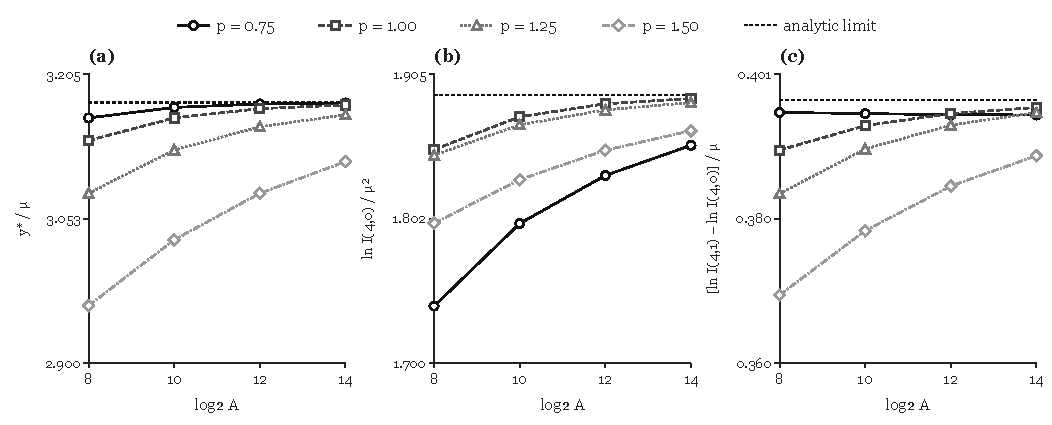
\includegraphics[width=\textwidth]{figures/heat-edge/figure.pdf}
 \caption{Finite heat-edge diagnostic at \(s=4\).
 The four degree laws use \(m\) equal to the positive even integer
 nearest \(A^\sigma\), for \(\sigma=0.75,1,1.25,1.5\), and
 \(A=256,1024,4096,16384\).
 Panels (a)--(c) show the saddle location divided by \(\mu\),
 \(\log I_{m,A}(4,0)/\mu^2\), and
 \([\log I_{m,A}(4,1)-\log I_{m,A}(4,0)]/\mu\).
 Dashed horizontal lines are the three analytic limits. All quantities
 are dimensionless and natural logarithms are used in (b)--(c).
 Each panel has a separately enlarged vertical range. The
 \(\sigma=0.75\) tilt sequence moves slightly away from its limit on
 this finite grid; convergence is not asserted from these plotted
 values. The letter \(p\) in the archived legend denotes \(\sigma\)
 here, not the pressure or the scale parameter \(p_0\).}
 \label{fig:edge-diagnostic}
\end{figure}

The archived calculation uses deterministic IEEE-754 binary64
quadrature, with 40\,001 grid points for the fine calculation and
20\,001 for comparison, and a log-phase drop of 48 to truncate the
integration interval. The plotting source, parameters, all 16 data
rows, and the numerical comparison report accompany the source
delivery. The two-resolution and tail-truncation comparisons measure
stability of this finite calculation. They provide no error enclosure
for every degree and scale. The limiting assertions and the
Navier--Stokes conclusions are justified by the analytic proofs.

\section{Limitations, open questions, and computational assistance}
\label{sec:discussion}

The combination of the results has a precise scope. Theorem
\ref{thm:ub-flux} gives a uniform bound over all finite packets in
one dyadic band. Theorem~\ref{thm:real-dyadic-lower} shows that the
spatial near-edge scale survives a real-valuedness restriction.
Theorem~\ref{thm:integer-slice} realizes a chosen slice in an exact
periodic heat shear. Theorem~\ref{thm:parabolic-shear} concerns one
explicit family throughout the full time interval. The last theorem
does not classify all packets satisfying the hypotheses of the first.

The transport flux here is signed. Its complete-time estimate uses
the scalar evolution equation and the cancellation of the two spatial
sides of the collar. Replacing it by an integral of the absolute
pointwise transport density changes the problem. Similarly, observing
only a central fibre changes the denominator; the full plateau
includes the transverse cross-section and the two tapering ends.

Several quantitative questions remain. The polynomial dependence on
\(q\) in the full-clock upper bound has not been optimized. A
time-integrated lower bound matching the entire uniform upper
coefficient remains open. The joint Chebyshev asymptotics proved here
stop at \(m=o(A^2)\). At substantially larger degree the dominant
Gaussian region and the integer-to-polynomial transfer change scale,
so a formal saddle calculation there needs a new uniform argument.
No such high-degree claim is used in this paper.

The exact shear form removes interactions present in general
three-dimensional flows. Passing from this model to multiple bands,
variable transport, or suitable weak solutions requires additional
estimates that have not been established here. A theorem about a
chosen periodic shear family cannot decide the global regularity or
singularity problem for arbitrary initial data.

\paragraph{Computer and AI assistance.}
OpenAI Codex assisted with manuscript drafting, literature retrieval,
proof organization, finite symbolic checks, and verification scripts.
The mathematical arguments used for the theorems are written in the
paper, and the specialized external inequalities are stated and
attributed. The numerical figure is an illustrative finite
calculation. The accompanying independent reviews are separate
automated review runs; external expert review remains outstanding.
The author remains responsible for the final submitted manuscript.

\paragraph{Reproducibility and version.}
This is the first complete consolidation of the accompanying
near-edge, dyadic-slice, and parabolic-shear research notes. The source
delivery contains a theorem-to-source map, a record of corrections
and supplementary arguments, the figure data and code, a build
recipe, and file checksums. Internal note identifiers occur in those
provenance files rather than as mathematical dependencies in the
proofs. The local review version has not been submitted to a journal
or to arXiv.


\begingroup
\small
\setlength{\bibsep}{4pt}
\bibliographystyle{plainnat}
\bibliography{references}
\endgroup
\end{document}
